\documentclass[11pt, article, one side]{memoir}

\settrims{0pt}{0pt} % page and stock same size
\settypeblocksize{*}{34.5pc}{*} % {height}{width}{ratio}
\setlrmargins{*}{*}{1} % {spine}{edge}{ratio}
\setulmarginsandblock{1in}{1in}{*} % height of typeblock computed
\setheadfoot{\onelineskip}{2\onelineskip} % {headheight}{footskip}
\setheaderspaces{*}{1.5\onelineskip}{*} % {headdrop}{headsep}{ratio}
\checkandfixthelayout


%-------- Packages --------%

\usepackage{mathtools}
\usepackage{amsthm}
%\usepackage{amssymb}
\usepackage{dutchcal}
\usepackage{newpxtext}
\usepackage[varg,bigdelims]{newpxmath}
%\usepackage{eucal}
%\usepackage[usenames,dvipsnames]{xcolor}
\usepackage{tikz}
%\usepackage[siunitx]{circuitikz}
%\usepackage{graphicx}
%\usepackage{outline}
%\usepackage{varwidth}
\usepackage[inline]{enumitem}
%\usepackage{ifthen}
%\usepackage[utf8]{inputenc} %allows non-ascii in bib file
\usepackage[bookmarks=true, colorlinks=true, linkcolor=blue!50!black,
citecolor=orange!50!black, urlcolor=orange!50!black, pdfencoding=unicode]{hyperref}
\usepackage[capitalize]{cleveref}
\usepackage[backend=biber, backref=true, maxbibnames = 10, style = alphabetic]{biblatex}
%\usepackage[framemethod=tikz]{mdframed}
%\usepackage{todonotes}

%-------- Package setup --------%

% cleveref %
  \newcommand{\creflastconjunction}{, and\nobreakspace} % serial comma

% biblatex %
  \addbibresource{Library20180913.bib} 

% makeidx %
  \makeindex 

% hyperref %
  \hypersetup{final}

% enumitem %
  \setlist{nosep}
  

% tikz %
  \usetikzlibrary{ 
  	cd,
  	math,
  	decorations.markings,
  	decorations.pathmorphing,
		decorations.pathreplacing,
  	positioning,
  	arrows.meta,
  	shapes,
		shadows,
		shadings,
  	calc,
  	fit,
  	quotes,
  	intersections,
    circuits,
    circuits.ee.IEC
  }
  
	\tikzcdset{arrow style=tikz, diagrams={>=To}}

% mdframed/tablefootnote%
% This makes \tablefootnote allow construction of footnotes that appear at bottom of page instead of inside frame


%\mdfdefinestyle{exerciseframe}{
%    linecolor=white!93!yellow,
%    backgroundcolor=white!93!yellow,
%    }


% amsthm %
  \theoremstyle{theorem}
  \newtheorem{theorem}[equation]{Theorem}
  \newtheorem{proposition}[equation]{Proposition}
  \newtheorem{corollary}[equation]{Corollary}
  \newtheorem{lemma}[equation]{Lemma}
  
  \theoremstyle{definition}
  \newtheorem{definition}[equation]{Definition}
  \newtheorem{notation}[equation]{Notation}
  \newtheorem{axiom}{Axiom}
  \newtheorem*{axiom*}{Axiom}
  
  \theoremstyle{remark}
  \newtheorem{example}[equation]{Example}
  \newtheorem{remark}[equation]{Remark}
  \newtheorem{warning}[equation]{Warning}
%  \newtheorem{exercise}[equation]{Exercise}

% Adjunctions
\newcommand{\adj}[5][30pt]{%[size] Cat L, Left, Right, Cat R.
\begin{tikzcd}[ampersand replacement=\&, column sep=#1]
  #2\ar[r, shift left=6pt, "#3"]
    \ar[l, phantom, "\Rightarrow"]\&
  #5\ar[l, shift left=6pt, "#4"]
\end{tikzcd}
}

\newcommand{\adjr}[5][30pt]{%[size] Cat R, Right, Left, Cat L.
\begin{tikzcd}[ampersand replacement=\&, column sep=#1]
  #2\ar[r, shift left=6pt, "#3"]\&
  #5\ar[l, shift left=6pt, "#4"]
  \ar[l, phantom, "\Leftarrow"]
\end{tikzcd}
}

  
%-------- Single symbols --------%
	
\DeclareSymbolFont{stmry}{U}{stmry}{m}{n}
\DeclareMathSymbol\fatsemi\mathop{stmry}{"23}

\DeclareFontFamily{U}{mathx}{\hyphenchar\font45}
\DeclareFontShape{U}{mathx}{m}{n}{
      <5> <6> <7> <8> <9> <10>
      <10.95> <12> <14.4> <17.28> <20.74> <24.88>
      mathx10
      }{}
\DeclareSymbolFont{mathx}{U}{mathx}{m}{n}
\DeclareFontSubstitution{U}{mathx}{m}{n}
\DeclareMathAccent{\widecheck}{0}{mathx}{"71}


%-------- Renewed commands --------%

\renewcommand{\ss}{\subseteq}

%-------- Other Macros --------%

\DeclarePairedDelimiter{\pair}{\langle}{\rangle}
\DeclarePairedDelimiter{\copair}{[}{]}
\DeclarePairedDelimiter{\floor}{\lfloor}{\rfloor}
\DeclarePairedDelimiter{\ceil}{\lceil}{\rceil}

\DeclarePairedDelimiter{\corners}{\ulcorner}{\urcorner}




\DeclareMathOperator{\Hom}{Hom}
\DeclareMathOperator{\Mor}{Mor}
\DeclareMathOperator{\dom}{dom}
\DeclareMathOperator{\cod}{cod}
\DeclareMathOperator*{\colim}{colim}
\DeclareMathOperator{\im}{im}
\DeclareMathOperator{\ob}{Ob}
\DeclareMathOperator{\Tr}{Tr}
\DeclareMathOperator{\dju}{\sqcup}
\DeclareMathOperator{\plpl}{+\!+}

\DeclareMathOperator{\const}{\mathtt{const}}

\newcommand{\Set}[1]{\mathrm{#1}}%a named set
\newcommand{\cat}[1]{\mathcal{#1}}%a generic category
\newcommand{\Cat}[1]{\mathsf{#1}}%a named category
\newcommand{\fun}[1]{\textit{#1}}%function
\newcommand{\Fun}[1]{\mathbf{#1}}%functor
\newcommand{\type}[1]{\texttt{#1}}

\newcommand{\id}{\mathrm{id}}
\newcommand{\cocolon}{:\!}
\newcommand{\iso}{\cong}
\newcommand{\too}{\longrightarrow}
\newcommand{\tto}{\rightrightarrows}
\newcommand{\To}[1]{\xrightarrow{#1}}
\newcommand{\Tto}[3][13pt]{\begin{tikzcd}[sep=#1, cramped, ampersand replacement=\&, text height=1ex, text depth=.3ex]\ar[r, shift left=2pt, "#2"]\ar[r, shift right=2pt, "#3"']\&{}\end{tikzcd}}
\newcommand{\Too}[1]{\xrightarrow{\;\;#1\;\;}}
\newcommand{\from}{\leftarrow}
\newcommand{\From}[1]{\xleftarrow{#1}}
\newcommand{\Fromm}[1]{\xleftarrow{\;\;#1\;\;}}
\newcommand{\surj}{\twoheadrightarrow}
\newcommand{\inj}{\rightarrowtail}
\newcommand{\wavyto}{\rightsquigarrow}
\newcommand{\lollipop}{\multimap}
\newcommand{\pr}{\mathrm{pr}}
\newcommand{\tickar}{\begin{tikzcd}[baseline=-0.5ex,cramped,sep=small,ampersand 
replacement=\&]{}\ar[r,tick]\&{}\end{tikzcd}}
\newcommand{\imp}{\Rightarrow}
\renewcommand{\iff}{\Leftrightarrow}
\renewcommand{\th}{\ensuremath{^\tn{th}}\ }
\newcommand{\down}{\mathbin{\downarrow}}
\newcommand{\then}{\mathbin{\scalebox{.8}{/\!\!/}}}
\newcommand{\op}{^\tn{op}}
\newcommand{\grph}[1]{{#1}_{\mathrm{Gr}}}

\newcommand{\tn}[1]{\textnormal{#1}}
\newcommand{\ol}[1]{\overline{#1}}
\newcommand{\ord}[1]{\underline{#1}}
\newcommand{\wt}[1]{\widetilde{#1}}
\newcommand{\wh}[1]{\widehat{#1}}
\newcommand{\ubar}[1]{\underaccent{\bar}{#1}}
\newcommand{\LMO}[2][over]{\ifthenelse{\equal{#1}{over}}{\overset{#2}{\bullet}}{\underset{#2}{\bullet}}}
\newcommand{\LTO}[2][\bullet]{\overset{\tn{#2}}{#1}}


\newcommand{\bb}{\mathbb{B}}
\newcommand{\nn}{\mathbb{N}}
%\newcommand{\PP}{\mathbb{P}}
\newcommand{\zz}{\mathbb{Z}}
\newcommand{\rr}{\mathbb{R}}
\newcommand{\oo}{\mathcal{O}}
\newcommand{\singleton}{\{1\}}
\newcommand{\powset}{\Fun{P}}
\newcommand{\upset}{\Fun{U}}

\newcommand{\foo}{\const{foo}}
\newcommand{\true}{\const{true}}
\newcommand{\false}{\const{false}}

\newcommand{\inv}{^{-1}}

\newcommand{\boxCD}[2][black]{\fcolorbox{#1}{white}{\begin{varwidth}{\textwidth}\centering #2\end{varwidth}}}

\newcommand{\lo}[2]{#1(\,\cdot\,)^{#2}}

\newcommand{\smset}{\Cat{Set}}
\newcommand{\smcat}{\Cat{Cat}}
\newcommand{\finset}{\Cat{Fin}}
\newcommand{\cont}{\Cat{Cont}}
\newcommand{\core}{\Fun{Core}}
\newcommand{\bun}{\Cat{Bun}}


\newcommand{\yon}{\mathcal{y}}
\newcommand{\poly}{\Cat{Poly}}
\newcommand{\dir}{\Cat{Dir}}
\newcommand{\ff}{\mathbb{F}}

\newcommand{\qand}{\quad\text{and}\quad}
\newcommand{\qqand}{\qquad\text{and}\qquad}

\newcommand{\inote}[1]{{\color{blue}David I.\ says: #1}}
\newcommand{\jnote}[1]{{\color{red}David J.\ says: #1}}


\newcommand{\cp}{\mathbin{\fatsemi}}

%%fakesubsubsection generators
%}

\linespread{1.15}
%\allowdisplaybreaks
\setsecnumdepth{subsubsection}
\settocdepth{subsection}
\setlength{\parindent}{15pt}
\setcounter{tocdepth}{2}
\setlength{\parskip}{0em}

\begin{document}

\title{Terms of the form $0^\yon$ in Dirichlet series\\contain significant content}

\author{David and David}

\maketitle
\begin{abstract}
One can think of power series or polynomials in one variable, such as $2\yon^3+\yon+5$, as functors from the category $\smset$ of sets to itself; these are known as polynomial functors. Denote by $\poly_\smset$ the category of polynomial functors on $\smset$ and natural transformations between them. The constants $0,1$ and operations $+,\times$ are the initial and terminal objects and the coproduct and product in $\poly_\smset$. 

Just as the polynomial functors are the copresheaves that can be written as sums of representables, one can express Dirichlet series, e.g.\ $\sum_{n=0}^\infty n^\yon$, as a coproduct of representable presheaves. Note that it is common to omit the $n=0$ term $0^\yon$, as it is ``just 0'', but it seems to us that this omission drops important category-theoretic content. Indeed, the category $\dir_\smset$ of Dirichlet functors has very nice formal properties---in fact it is an elementary topos---so we may take seriously the fact that the object $0^\yon$---the representable functor on the empty set---is decidedly not $0$.

We also show that there is a double category, useful in applications, whose vertical category is isomorphic to $\poly$ and whose horizontal category is isomorphic to $\dir$.
\end{abstract}

Polynomials $P(\yon)$ and finite Dirchlet series $D(\yon)$ in one variable $\cat{y}$, with natural number coefficients $a_i\in\nn$, are respectively functions of the form
\[
  P(\yon)=a_n\yon^n+\cdots+a_2\yon^2+a_1\yon^1+a_0\yon^0
  \qqand
  D(\yon)=a_nn^\yon+\cdots+a_22^\yon+a_11^\yon+a_00^\yon.
\]
There are of course infinite versions of the above, but in this note we work entirely in the topos $\finset$ of finite sets, to keep things simple. Similar considerations hold for infinite Dirichlet series or power series, with an appocone get them and much more by replacing $\finset$ with $\smset$ everywhere.

\chapter{The categories $\poly$ and $\dir$}
Recall that a \emph{co-representable functor} $\finset\to\finset$ is one of the form $\finset(n, -)$ for some finite set $n=\{`1', `2',\ldots,`n'\}$. We denote this functor by $\yon^n$ and say it is \emph{represented by} $n\in\finset$. Similarly, a \emph{(contra-) representable functor} $\finset\op\to\finset$ is contravariant functor of the form $\finset(-,n)$; we denote this functor by $n^\yon$.
\begin{figure}
\[
  \yon^n \coloneqq \finset(n,-)
  \qqand
  n^\yon\coloneqq\finset(-,n).
\]
  \caption{The pure power polynomial $\yon^n$ and the pure exponential Dirichlet series $n^\yon$ are the representable functors in $\poly$ and $\dir$.}
\end{figure}
The functors $\yon_-$ and $\yon^-$ are the covariant and contravariant Yoneda embeddings.

Note that the functor $0^\yon\not\cong 0$ is not the initial object; it is given by
\[
0^\yon(s)=
\begin{cases}
1&\tn{ if } s=0\\
0&\tn{ if } s\geq1.
\end{cases}
\]
The coefficient $p_0$ of $1$ in a polynomial $P$ is called its constant term. We refer to the coefficient $d_0$ of $0^\yon$ in a Dirichlet series $D$ as its \emph{exceptional term}.

\begin{example}
The reader can determine which finite Dirichlet series $D(\yon)$ has the following terms
\[
\begin{array}{c|ccccccc}
\yon&
\cdots&
5&
4&
3&
2&
1&
0
\\\hline
D(\yon)&
\cdots&
96&
48&
24&
12&
6&
7
\end{array}
\]
Hint: its exceptional term is $4$.
\end{example}

\paragraph{Polynomial and Dirichlet functors.}
A \emph{polynomial functor} \cite{GambinoKock} is a functor $P\colon\finset\to\finset$ that can be expressed as a finite sum of co-representable functors. Similarly, we define a \emph{Dirichlet functor} to be a functor $D\colon\finset\op\to\finset$ that can be expressed as a finite sum of representable presheaves (contravariant functors):
\begin{equation}\label{eqn.finite_sum}
  P=\sum_{i=1}^{P(1)}\yon^{p_i}
  \qqand
  D=\sum_{i=1}^{D(0)}(d_i)^\yon.
\end{equation}
That is $P(X)=\sum_{i=1}^{P(1)}\finset(p_i,X)$ and $D(X)=\sum_{i=1}^{D(0)}\finset(X,d_i)$.

For any small category $C$, let $\finset^C$ denote the category whose objects are the functors $C\to\finset$ and whose morphisms are the natural transformations between them.

\begin{definition}\label{def.poly_dir}
The \emph{category of polynomial functors}, denoted $\poly$, is the full subcategory of $\finset^\finset$ spanned by finite sums $P$ of representable functors. The \emph{category of Dirichlet functors}, denoted $\dir$, is the full subcategory of $\finset^{(\finset\op)}$ spanned by the finite sums $D$ of representable presheaves.
\end{definition}

\begin{lemma}
The number of polynomial maps $P\to Q$ and Dirichlet maps $D\to E$ are
\[
  [P, Q]\coloneqq\prod_{i\in P(1)}Q(p_i)
  \qqand
  [D, E]\coloneqq\prod_{i\in D(0)}E(d_i),
\]
\end{lemma}

\begin{example}
Let $P=2\yon^2$, $Q=\yon+1$, and let $D=2\cdot2^\yon$ and $E=1+0^\yon$. Then there are nine ($9$) polynomial morphisms $P\to Q$, zero ($0$) polynomial morphisms $Q\to P$, one ($1$) Dirichlet morphism $D\to E$, and eight ($8$) Dirichlet morphiisms $E\to D$.
\end{example}

\begin{remark}\label{rem.products_coproducts}
Sums and products of polynomials in the usual algebraic sense agrees exactly with sums and products in the categorical sense: if $P$ and $Q$ are polynomials, i.e.\ objects in $\poly$, then their coproduct is $P+Q$ and their product is $PQ$. The same is true for $\dir$: sums and products of finite Dirichlet series in the usual sense agrees exactly with sums and products in the categorical sense.
\end{remark}

\paragraph{Formal structures.}
There are adjoint quadruples and sextuples as follows, labeled by where they send objects $n\in\finset$, $P\in\poly$, $D\in\dir$:
\begin{equation}\label{eqn.adjoints_galore}
\begin{tikzcd}[column sep=60pt]
  \finset
  	\ar[r, shift left=7pt, "n" description]
		\ar[r, shift left=-21pt, "n\yon^1"']&
  \poly
  	\ar[l, shift right=21pt, "P(0)"']
  	\ar[l, shift right=-7pt, "P(1)" description]
	\ar[l, phantom, "\Leftarrow"]
	\ar[l, phantom, shift left=14pt, "\Rightarrow"]
	\ar[l, phantom, shift right=14pt, "\Rightarrow"]
\end{tikzcd}
\hspace{1in}
\begin{tikzcd}[column sep=60pt]
  \finset
  	\ar[r, shift left=7pt, "n\cdot 0^\yon" description]
		\ar[r, shift left=-21pt, "n" description]
		\ar[r, shift left=-49pt, "n^\yon"']&
  \dir
  	\ar[l, shift right=21pt, "d_0"']
  	\ar[l, shift right=-7pt, "D(0)" description]
		\ar[l, shift right=-35pt, "D(1)" description]
	\ar[l, phantom, shift right=14pt, "\Leftarrow"]
	\ar[l, phantom, shift right=0pt, "\Rightarrow"]
	\ar[l, phantom, shift right=-14pt, "\Leftarrow"]
	\ar[l, phantom, shift right=-28pt, "\Rightarrow"]
	\ar[l, phantom, shift right=-42pt, "\Leftarrow"]
\end{tikzcd}
\end{equation}
All six of the functors out of $\finset$ are fully faithful. The inclusion $d_0\to D(0)$ of the exceptional terms is natural and induces three other natural transformations on $\finset$ and $\dir$, the most important of which we label $\pi_D$
\begin{equation}\label{eqn.obtain_pi}
d_0\to D(0),\qquad
n{\cdot}0^\yon\to n,\qquad
D(1)\To{\pi_D} D(0),\qquad
n\to n^\yon.
\end{equation}

There are also two-variable adjunctions $\finset\times\poly\to\poly$ and $\finset\times\dir\to\dir$. Indeed, for $n\in\finset$ and $P,Q\in\poly$ (respectively $D,E\in\dir$), we have
\begin{gather*}
\poly(nP,Q)\cong\poly(P,Q^n)\cong\finset(n,[P,Q]),\\
\dir(nD,E)\cong\dir(D,E^n)\cong\finset(n,[D,E]).
\end{gather*}

Each of the categories $\poly$ and $\dir$ has pullbacks, which we denote using ``fiber product notation'' $A\times_CB$. We can use pullbacks in combination with monads $\eta_P\colon P\to P(1)$ and $\eta_D\colon D\to D(0)$ arising from \cref{eqn.adjoints_galore} to recover \cref{eqn.finite_sum}:
\[
  P=\sum_{i=1}^{P(1)}P\times_{P(1)}`i'
  \qqand
	D=\sum_{i=1}^{D(0)}D\times_{D(0)}`i'.
\]
\begin{remark}
The Yoneda embedding for $\poly$ also has a left adjoint given by \emph{global sections}
\[
	\adjr[50pt]{\finset\op}{n\mapsto\yon^n}{\prod_ip_i\mapsfrom P}{\poly},
\]
though it appears to be less important than the analogue $D\mapsto D(1)$ for $\dir$.
\end{remark}

\paragraph{Dirichlet transform.}
There is a bijection between the respective object-sets of these two categories
\begin{align}
\nonumber
	\ob(\poly)&\To{\cong}\ob(\dir)\\\label{eqn.poly_dir}
	\sum_{i=1}^n\yon^{k_i}&\mapsto\sum_{i=1}^n (k_i)^\yon.
\end{align}
We call this mapping the \emph{Dirichlet transform} and denote it using an over-line $P\mapsto \overline{P}$.

\begin{proposition}\label{prop.poly_function}
There is a one-to-one correspondence between the set of polynomials in one variable, the set of finite Dirichlet series, and the set of (isomorphism classes of) functions $\pi\colon s\to t$ between finite sets.
\end{proposition}
\begin{proof}
We already established a bijection $P\mapsto\overline{P}$ between polynomials and finite Dirichlet series in \cref{eqn.poly_dir}.

Given a finite Dirichlet series $D$, we have a function $\pi_D\colon D(1)\to D(0)$ as in \cref{eqn.obtain_pi}. And given a function $\pi\colon s\to t$, define $D_\pi\coloneqq\sum_{i=1}^t(d_i)^\yon$, where $d_i\coloneqq\pi\inv(i)$ for each $1\leq i\leq t$. (N.B.\ Rather than constructing $D_\pi$ from $\pi$ by hand, one could instead use a certain orthogonal factorization system on $\dir$.)

It is easy to see that the roundtrip on Dirichlet series is identity, and that the round-trip for functions is a natural isomorphism.
\end{proof}

\begin{example}
The polynomial $2\yon^3+\yon^2+3$ and the Dirichlet series $2{\cdot}3^\yon+2^\yon+3{\cdot} 0^\yon$ correspond to the function
\begin{equation}\label{eqn.bundle}
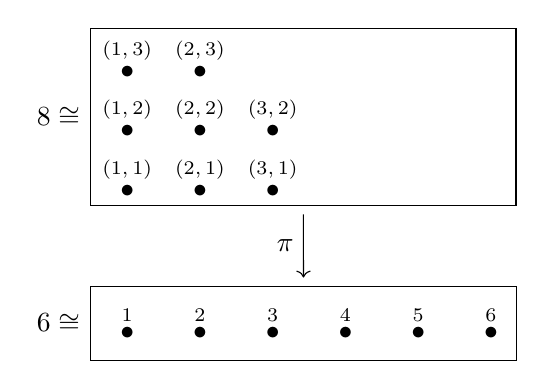
\begin{tikzpicture}[x=.5cm, y=.35cm, every label/.style={font=\scriptsize}, baseline=(f)]
	\node[label={[above=-5pt]:$1$}] (Ya) {$\bullet$};
	\node[right=1 of Ya,  label={[above=-5pt]:$2$}] (Yc) {$\bullet$};
	\node[right=1 of Yc,  label={[above=-5pt]:$3$}] (Yd) {$\bullet$};
	\node[right=1 of Yd,  label={[above=-5pt]:$4$}] (Ye) {$\bullet$};
	\node[right=1 of Ye,  label={[above=-5pt]:$5$}] (Yf) {$\bullet$};
	\node[right=1 of Yf,  label={[above=-5pt]:$6$}] (Yg) {$\bullet$};
	\node[draw, inner ysep=4pt, fit={($(Ya)+(-1em,3ex)$) (Yg)}] (Y) {};
	\node[left=0 of Y] (Ylab) {$6\cong$};
%
  \node[above=4 of Ya, label={[above=-5pt]:$(1,1)$}] (X11) {$\bullet$};
  \node[above=1 of X11, label={[above=-5pt]:$(1,2)$}] (X12) {$\bullet$};
  \node[above=1 of X12, label={[above=-5pt]:$(1,3)$}] (X13) {$\bullet$};
%
  \node[above=4 of Yc, label={[above=-5pt]:$(2,1)$}] (X31) {$\bullet$};
  \node[above=1 of X31, label={[above=-5pt]:$(2,2)$}] (X32) {$\bullet$};
  \node[above=1 of X32, label={[above=-5pt]:$(2,3)$}] (X33) {$\bullet$};
%
  \node[above=4 of Yd, label={[above=-5pt]:$(3,1)$}] (X41) {$\bullet$};
  \node[above=1 of X41, label={[above=-5pt]:$(3,2)$}] (X42) {$\bullet$};
  \node [above=4 of Yg] (xend) {};
	\node[draw, inner ysep=3pt, fit={($(X13)+(-1em,3ex)$) ($(xend)+(.4,0)$)}] (X) {};
	\node[left=0 of X] {$8\cong$};
%
	\draw[->, shorten <=3pt, shorten >=3pt] (X) to node[left] (f) {$\pi$} (Y);
\end{tikzpicture}
\end{equation}
\end{example}

We can think of a function $\pi\colon s\to t$, e.g.\ that shown in \eqref{eqn.bundle}, as a \emph{bundle} of fibers $\pi\inv(i)$, one for each element $`i'\in t$. In \cref{def.sheaves_bundles} we define two different notions of morphism between them, which correspond to maps in $\poly$ and $\dir$.

For any function $f\colon t\to t'$ and function $\pi'\colon s'\to t'$, denote by $f^*(\pi')$ the pullback function as shown
\[
\begin{tikzcd}
	s\times_{t'}s'\ar[r]\ar[d, "f^*(\pi')"']&
	s'\ar[d, "\pi"]\\
	t\ar[r, "f"']&
	t'\ar[ul, phantom, very near end, "\lrcorner"]
\end{tikzcd}
\]

\begin{definition}\label{def.sheaves_bundles}
Let $\pi\colon s\to t$ and $\pi'\colon s'\to t'$ be functions between finite sets.
\begin{itemize}
	\item a \emph{bundle morphism} consists of a pair $(f,f_\sharp)$ where $f\colon t\to t'$ is a function and $f_\sharp\colon \pi\to f^*(\pi')$ is a morphism in the slice category over $t$;
	\item a \emph{container morphism} consists of a pair $(f,f^\sharp)$ where $f\colon t\to t'$ is a function and $f^\sharp\colon f^*(\pi')\to \pi$ is a morphism in the slice category over $t$.
\end{itemize}
\begin{equation}\label{eqn.bund_cont_maps}
\begin{tikzcd}
s\ar[dr, bend right=40pt, "\pi"']&[-5pt]
t\times_{t'}s'\ar[r]\ar[d, "f^*\pi'"']\ar[from=l, "f_\sharp"]&
s'\ar[d, "\pi'"]\\&
t\ar[r, "f"']&
t'\ar[ul, phantom, very near end, "\lrcorner"]
\end{tikzcd}
\hspace{.75in}
\begin{tikzcd}
s\ar[dr, bend right=40pt, "\pi"']&[-5pt]
t\times_{t'}s'\ar[r]\ar[d, "f^*\pi'"']\ar[l, "f^\sharp"']&
s'\ar[d, "\pi'"]\\&
t\ar[r, "f"']&
t'\ar[ul, phantom, very near end, "\lrcorner"]
\end{tikzcd}
\end{equation}
Define $\bun$ (resp.\ $\cont$) to be the category for which an object is a function between finite sets and a morphism is a bundle morphism (resp.\ container morphism).
\end{definition}

\begin{remark}\label{rem.dir_fin2}
It is easy to check that $\bun\cong\finset^2$ is the category of morphisms and commuting squares in the category of finite sets. Next we show that it is also isomorphic to the category of Dirichlet functors from \cref{def.poly_dir}.

The reader familiar with basic algebraic geometry will see an analogy between morphisms in $\cont$ and homomorphisms of ringed spaces. The name \emph{container} comes from computer science; see \cite{**}.
\end{remark}

\begin{theorem}\label{thm.equivs}
We have equivalences of categories
\[
\poly\cong\cont
\qqand
\dir\cong\bun.
\]
\end{theorem}
\begin{proof}
The functors $P_-\colon\cont\to\poly$ and $D_-\colon\bun\to\dir$ are defined on each object $\pi\colon s\to t$ by the formula $\pi\mapsto P_\pi$ and $\pi\mapsto D_\pi\coloneqq\overline{P_\pi}$ as in \cref{prop.poly_function}. For each $1\leq i\leq t$, denote the fiber of $\pi$ over $i$ by $k_i\coloneqq\pi\inv(i)$.

For any set $X$, consider the unique map $X!\colon X\to 1$. Applying $P_-$ and $D_-$ to it, we obtain the corresponding representable: $P_{X!}\cong\yon^X$ and $D_{X!}\cong X^\yon$. We next check that
 \begin{gather*}
  \poly(P_{X!},P_\pi)\cong 
  P_\pi(X)=
  \sum_{i=1}^{t}X^{k_i}\cong
  \cont(X!, \pi),
  \\
  \dir(D_{X!}, D_\pi)\cong 
  D_\pi(X)=
  \sum_{i=1}^{t}(k_i)^X\cong
  \bun(X!, \pi).
\end{gather*}
In both lines, the first isomorphism is the Yoneda lemma and the second is a computation. Thus we define $P_-$ on morphisms by sending $f\colon\pi\to\pi'$ in $\cont$ to the natural transformation with $X$-component $\cont(X!,f)\colon\cont(X!,\pi)\to\cont(X!,\pi')$, which is clearly natural in $X$. We define $D_-$ on morphisms similarly: for $f$ in $\bun$, use the natural transformation $\bun(-!,f)$.

By definition, every object in $\poly$ and $\dir$ is a coproduct of representables, so to complete the proof one first checks that coproducts in $\cont$ and $\bun$ are taken pointwise:
\[
(\pi\colon s\to t)+(\pi'\colon s'\to t')\cong(\pi+\pi')\colon (s+s')\to (t+t').
\]
and then that $P_{\pi+\pi'}=P_\pi+P_{\pi'}$ and $D_{\pi+\pi'}=D_\pi+D_{\pi'}$; see \cref{eqn.Ppi}.
\end{proof}

\begin{corollary}
$\dir$ is an elementary topos.
\end{corollary}
\begin{proof}
For any finite category $C$, the functor category $\finset^C$ is an elementary topos. The result now follows from \cref{rem.dir_fin2,thm.equivs}.
\end{proof}

\chapter{The $\poly-\dir$ double category $\ff$}

There is a double category $\ff$ whose objects are functions between finite sets, whose vertical category is $\poly$, whose horizontal category is isomorphic to $\bun$. This double category shows up in the theory of mode-dependent dynamical systems, though we save this for future work.

The double category $\ff$ will be thin, meaning that for every square there is at most one 2-cell filler. Squares (with or without filler) can be drawn as \emph{bevelled squares}:
\[
\begin{tikzcd}[sep=large]
&[-35pt]
\overline{P}\ar[r, "f"]&
\overline{Q}\\[-25pt]
P\ar[d, "g"']\arrow[ur, no head]&&&[-35pt]\ar[ul, no head]\ar[d, "h"]
Q\\
P'\ar[dr, no head]&&&
Q'\ar[dl, no head]\\[-25pt]&
\overline{P}'\ar[r, "f'"']&
\overline{Q}'
\end{tikzcd}
\]
where $g,h$ are in $\poly$ and $f,f'$ are in $\dir$, and where the unlabeled line segments are just tracking Dirchlet transforms. Thus to define $\ff$, it remains to give the conditions for when a filler exists for $(f,f',g,h)$; there will be two.

Suppose first that $P=\yon^m$ is a pure power, i.e.\ $P(1)=1$; this is the case iff its Dirichlet transform $\overline{P}=m^\yon$ is a pure exponential $D(0)=1$. In that case $g$ picks out an element $g(1)\in P'(1)=\ol{P}'(0)$ and $f$ picks out an element $f(1)\in \ol{Q}(0)=Q(1)$. Let $m'$ be the finite set corresponding to the exponent on $g(1)$ and let $n$ be the finite set corresponding to the base on $f(1)$
\[
  \yon^{m'}\coloneqq P'\times_{P(1)}g(1)
  \qqand
  n^\yon\coloneqq\ol{Q}\times_{\ol{Q}(0)}f(1)
\]
Then $f'$ picks out an element $f'(g(1))\in\ol{Q}'(0)=Q'(1)$ and $h$ picks out an element $h(f(1))\in Q'(1)=\ol{Q}'(0)$. The first condition is that $h(f(1))=f'(g(1))$. We may then define $n'$ to be the corresponding finite set, so that
\[
  \yon^{n'}= Q'\times_{Q'(1)}f'(g(1))
  \qqand
  (n')^\yon=\ol{Q}'\times_{\ol{Q}'(0)}h(f(1))
\]
By \cref{eqn.bund_cont_maps} we then obtain four maps
\begin{align*}
	g^\sharp&\colon\yon^m\to\yon^{m'}&
	f_\sharp&\colon m^\yon\to n^\yon\\
	f'_\sharp&\colon(m')^\yon\to(n')^\yon&
	h^\sharp&\colon\yon^{n}\to\yon^{n'}
\end{align*}
and by the Yoneda lemma, these induce composable functions
\[
  m'\To{g^\sharp} m\To{f_\sharp} n
  \qqand
  m'\To{f'_\sharp} n'\To{h^\sharp} n
\]
The second condition is that these are the same function $m'\to n$. 

In general, $P$ may not be a pure power, but it is a coproduct over $i\in P(1)$ of pure powers $\yon^{p_i}$. We say that a beveled square has a filler iff the above two conditions hold for each summand.

It is easy to check that we indeed have a double category.
\begin{theorem}
There is a thin double category whose objects are functions $\pi\colon s\to t$, whose vertical category is $\poly\cong\cont$, whose horizontal category is $\dir\cong\bun$, and for which 2-cells are defined as above.
\end{theorem}



%Given a combinatorial species $A : \textbf{Fin}^{\cong} \to \smset$, its
%\emph{Cauchy generating functor} $X \mapsto \sum_{n : \textbf{Fin}} A_n \times X^n/n!$
%is the left Kan extension of $A$ along the inclusion $\textbf{Fin}^{\cong}
%\hookrightarrow \smset$, and the \emph{Dirichlet generating functor} $S \mapsto
%\sum_{n : \textbf{Fin}} A_n n^S/n!$ is the left Kan extension of $A$ along the
%inclusion $\textbf{Fin}^{\cong} \hookrightarrow \smset^{\text{op}}$. These give
%functors
%\[
%  \begin{tikzcd}
%    & \textbf{CombSpecies} \arrow[dr, "|\cdot|_{\dir}"] \arrow[dl, "|\cdot|_{\poly}"']& \\
%    \poly & & \dir
%  \end{tikzcd}
%\]
%
%The Cauchy product $\otimes_{\poly}$ of combinatorial species is given by Day
%convolution from $+ : \textbf{Fin}^{\cong} \times \textbf{Fin}^{\cong}$, and
%$|\cdot|_{\poly}$ sends $\otimes_{\poly}$ to the cartesian product. On the
%other hand, the Dirichlet product $\otimes_{\dir}$ of combinatorial species is
%given by Day convolution from $\times : \textbf{Fin}^{\cong} \times
%\textbf{Fin}^{\cong}$, and this is sent by $|\cdot|_{\dir}$ to the cartesian
%product. This gives us an interpretation of the generating \emph{functors}
%associated to a species in which sum is coproduct and product is cartesian
%product -- the difference between the Cauchy generating functor and the
%Dirichlet generating functor is that the latter is contravariant.



\end{document}